\chapter{Résultats}


\paragraph{Resultats théoriques: }
Suite à l'apprentissage du réseau de neurone, nous avons obtenu une précision de 58\% sur les données de tests 

\begin{figure}[!ht]
  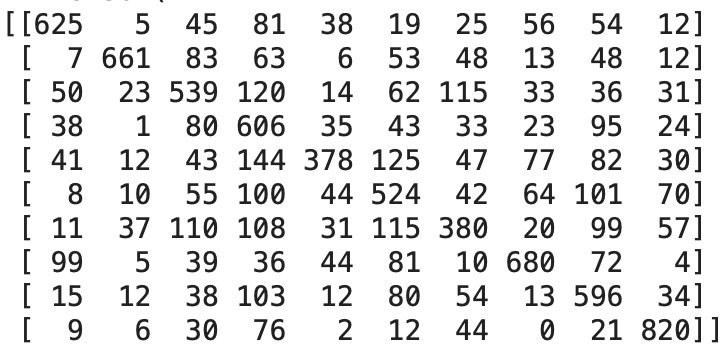
\includegraphics[width=0.5\textwidth]{confusion_matrix1}
  \centering
  \caption{Workflow Iteratif}
  \label{graph:confusion_matrix1}
\end{figure}


\begin{figure}[!ht]
  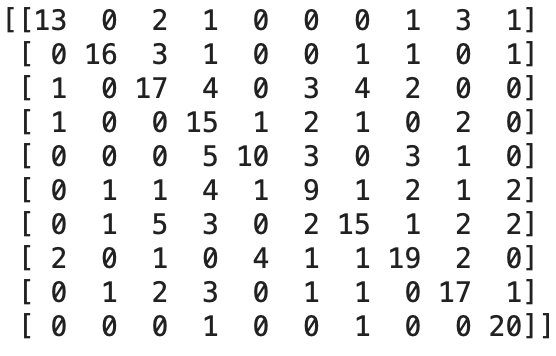
\includegraphics[width=0.5\textwidth]{confusion_matrix2}
  \centering
  \caption{Workflow Iteratif}
  \label{graph:confusion_matrix2}
\end{figure}


\paragraph{Résultats expérimentaux: } Pour tester nos résultats nous avons déployé le réseau de neurone sur la carte Nucleo à l'aide 
de l'IDE Arduino. Pour cela nous avons utilisé le même projet Arduino que dans le Lab 5, lors de la réalisation du CNN à partir du
jeu de donnée Google Speech Commons.



• Presentation of the results obtained, and the experimental setup to test the generalization of
the training to real data (not the ones of the dataset).


\paragraph{Performance}
\paragraph{Mémoire}
\paragraph{Latence}
\paragraph{Energie}
• Analysis of the result of your project on the following criteria
o Performance (accuracy on train, test and on real data after quantization)
o Memoryfootprint
o Latency
o Energy consumption and battery lifetime analysis (provide assumptions of your
estimation)

